\section{Design}

\subsection{Design Procedure}
Our design consists of four different subsystems, each with their own functions and requirements. At the center of the system is the control subsystem consisting of the ESP-32 microcontroller along with some simple logic for controlling the LEDs. The goal of this subsystem is to establish communication with the sensors, receive the necessary data from them, determine which hand gesture is being activated, and activate the corresponding LEDs. The main design decisions that we had to make for the control subsystem were software related as the circuit is quite simple. We decided to simplify the algorithm for detecting the gestures due to some time constraints with the PCB order waves along with a problematic ESP-32 DevKit. We originally wanted to devise an algorithm that utilized all three sensors on the IMU, but ultimately decided that it would be too difficult to program, and we found that the magnetometer was all that was necessary to accurately detect the gestures.

The original plan was to use an IMU on each arm, but this approach proved to be difficult in terms of programming. Instead, we used one on the waist, which ensures that one of the IMUs is always stable. Then, we just take the difference in angles between the two IMUs, and set ranges for each hand gesture. We also had to discard our PCBs for our IMUs as we were unsuccessful in soldering the small IMUs onto the board. Therefore we decided to continue with the breakout boards. 

For the power subsystem, we decided that the system should last at least one hour. We determined the current required to power the system to be 1864.2A total, so we needed a battery that could supply 5V with a capacity larger than 1864mAh, in addition to being rechargeable. The battery we used for the power subsystem was a 3000mAh 4.8V NiMH battery that provided ample voltage and current to power the LEDs. During the Design review, using an LED Driver was recommended to get a constant current to the LEDs. We researched several drivers and found one that fits the requirements. However, we also tested the LEDs without the driver, and the brightness was sufficient. The plan was to add the driver to get slightly brighter LEDs, but the driver only works with a PCB, and we were unable to get the LED drivers to function from the first and third order PCBs. Ultimately we decided to discard the LED driver in order to simplify the PCB and increase the odds of it functioning properly. We decided that a working PCB was more important than a slightly brighter LED.

\subsection{Design Details}
The LM317 datasheet \cite{TI2023} provides us with equation (1) which relates the output voltage to the resistances of $R_1$ and $R_2$ when using the schematic in figure \ref{fig:power_sub}

\begin{equation}
V_0 = V_{REF} \left(1 + \frac{R_2}{R_1}\right) + I_{ADJ} \times R_2 \quad \cite{TI2023}
\end{equation}

Where $R_1$ and $R_2$ control the output voltage of the linear voltage regulator, and $V_{\text{REF}}$ and $I_{\text{ADJ}}$ are given to be 1.25V and 50$\mu$ A respectively. Using this equation, we were able to find the resistor values necessary to achieve an output of 3.3V, which are $R_1 = 314.2 \Omega$ and $R_2 = 512 \Omega$. Note that we also have a linear voltage regulator which outputs 1.8V, which we added with the intent of making our own IMU PCB, but we ended up using a breakout board which takes in 3.3V.

\begin{figure}[ht]
    \centering
    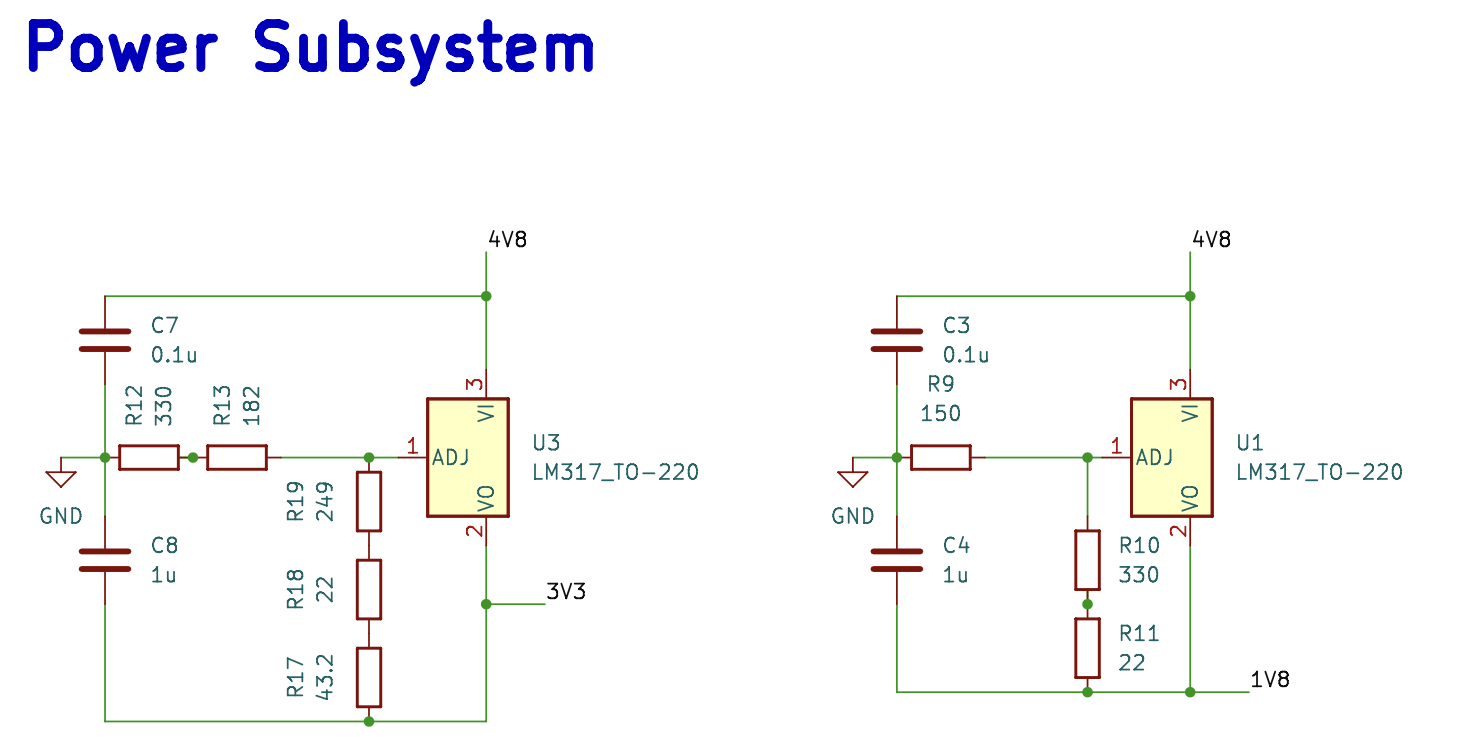
\includegraphics[width=0.8\textwidth]{images/power_sub.png}
    \caption{Schematic of the power subsystem}
    \label{fig:power_sub}
\end{figure}
\newpage
The control unit in figure \ref{fig:control_sub} consists of the ESP32-S3 \cite{EspressifESP32} which we use to control our entire system. We needed to add a programming circuit for it and ensure it has the proper connections to all the other subsystems.

\begin{figure}[ht]
    \centering
    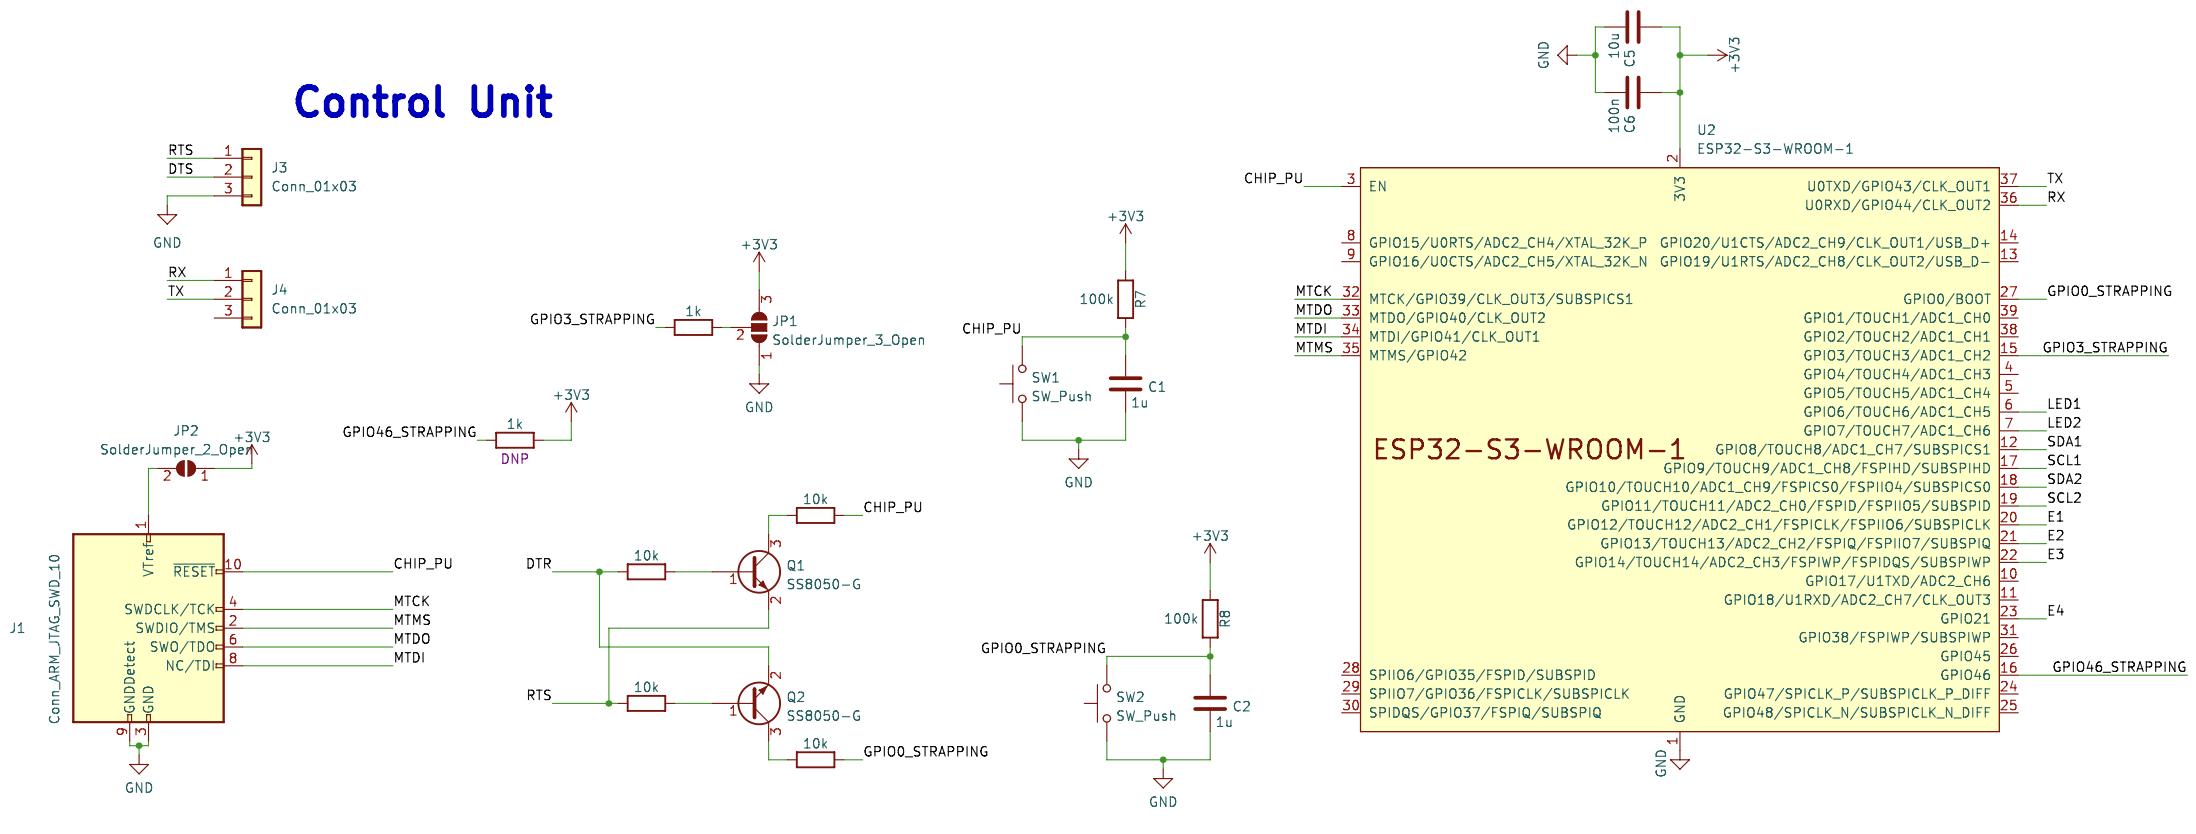
\includegraphics[width=1.0\textwidth]{images/control_sub.png}
    \caption{Schematic of the control subsystem}
    \label{fig:control_sub}
\end{figure}

Our LED subsystem in figure \ref{fig:LED_sub} was intended to use an LED driver, so we designed a circuit for it which we have on our pcb. Due to time constraints however we did not have enough time to test it and ended up hotwiring the LEDs to bypass the LED driver.
\begin{figure}[ht]
    \centering
    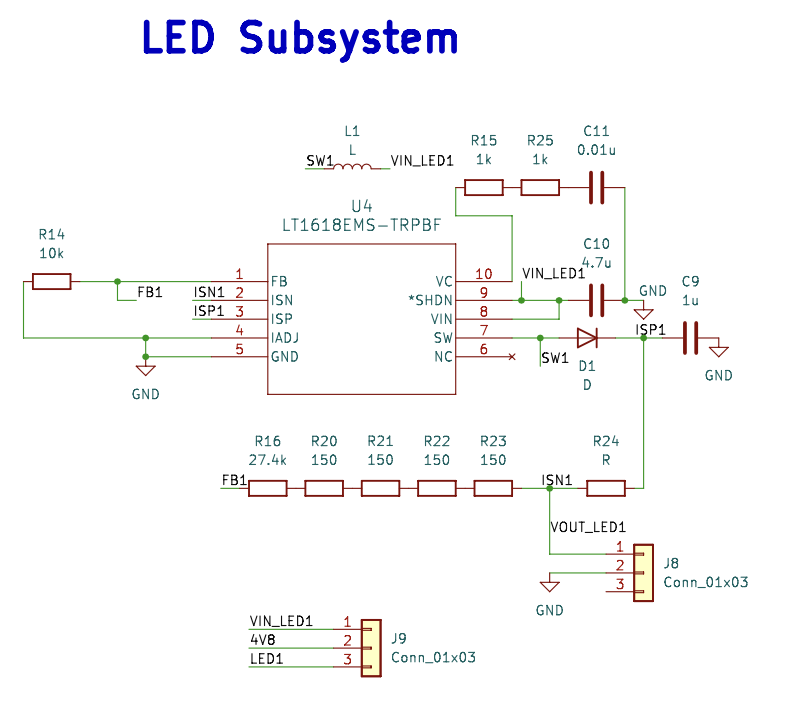
\includegraphics[width=0.7\textwidth]{images/LED_sub.png}
    \caption{Schematic of the LED subsystem}
    \label{fig:LED_sub}
\end{figure}
\newpage
The sensor subsystem in figure \ref{fig:IMU_sub} consists of the ICM-20948 IMU which we use to detect the hand gestures. This schematic shows the suggested connections \cite{invensense2016icm20948} for the IMU to communicate via I2C with the ESP32. Unfortunately, we were unable to get the IMU to work with the ESP32, so we had to use the breakout board which has a built-in voltage regulator and I2C communication.

\begin{figure}[ht]
    \centering
    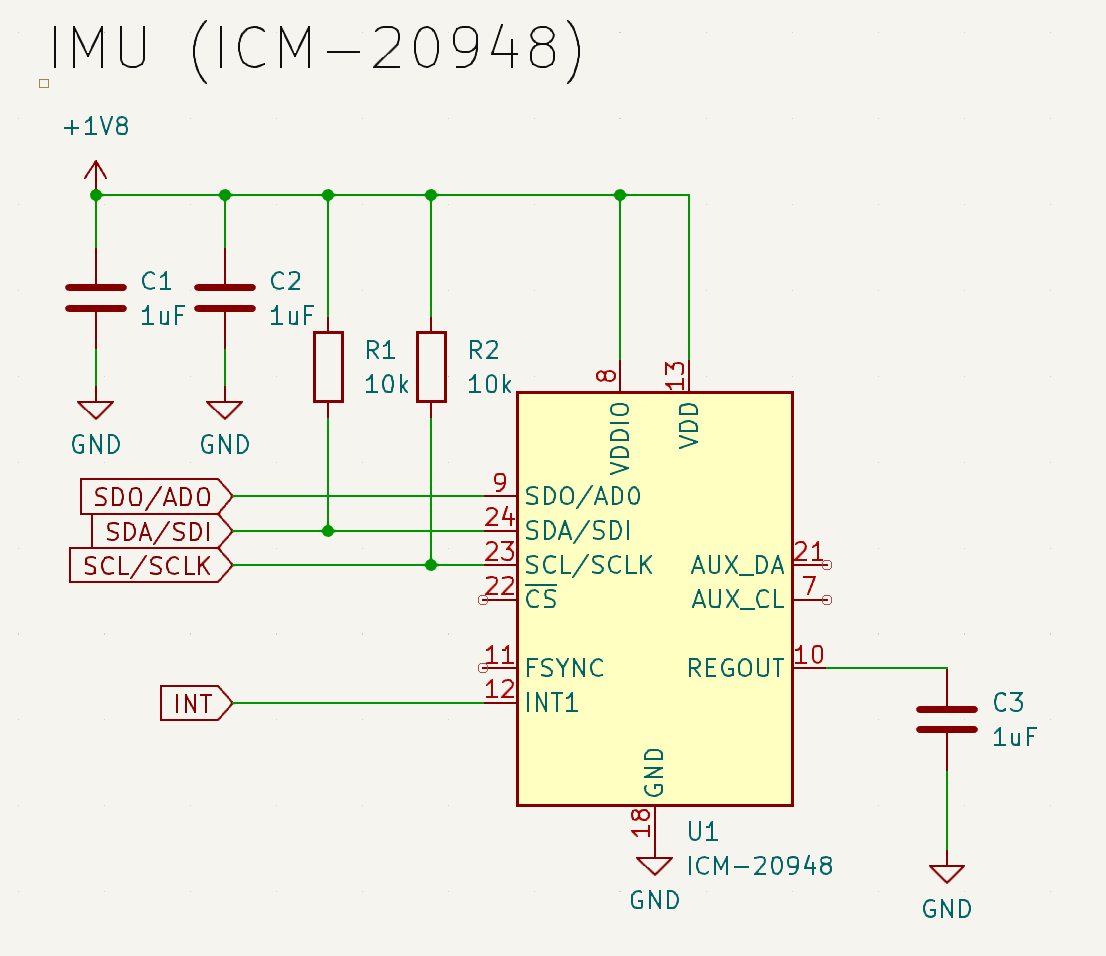
\includegraphics[width=0.75\textwidth]{images/IMU_schematic.png}
    \caption{Schematic of the sensor subsystem}
    \label{fig:IMU_sub}
\end{figure}
In order to power the system, we used a 3000mAh 4.8V NiMH battery from Panasonic \cite{panasonic2023datasheet}. As shown in table \ref{tab:current_draw}, our total current draw is 1864.2 mA so our estimated battery life of the system is $3000 \text{ mAh} / 1864.2 \text{ mA} = 1.61 \text{ hours}$. 
\begin{table}[h]
    \centering
    \caption{Current Draw of System Components}
    \label{tab:current_draw}
    \begin{tabular}{|l|l|}
        \hline
        \textbf{Description} & \textbf{Value} \\
        \hline
        ESP-32 worst case current draw & 355 mA \\
        \hline
        2x ICM-20948 IMU & 4.6 mA each = 9.2 mA total \\
        \hline
        2x LED strip & 750 mA each = 1500 mA total \\
        \hline
        \textbf{Total current draw} & 1864.2 mA \\
        \hline
    \end{tabular}
\end{table}

\section*{Heat tolerance for battery}
\begin{itemize}
    \item Total Internal Impedance = $4\, \text{m}\Omega \times 4 = 16\, \text{m}\Omega$.
    \item $I = 2\, \text{A}$
    \item Time = 3600 seconds
    \item Mass = 0.228 kg for 4 cells
    \item Specific Heat Capacity: $900\, \text{J/kg}^\circ \text{C}$
    \item Total Heat Generated = $I^2 \times R \times \text{time} = 230.4\, \text{J}$
    \item Change in temp = $\frac{\text{Heat}}{\text{mass} \times \text{specific heat capacity}} = 1.123^\circ \text{C}$

\end{itemize}
Assuming an ambient temperature of $25^\circ \text{C}$, the temperature of the battery will be around $26.123^\circ \text{C}$ after one hour of operation. This is well within the operating temperature of the battery, so we can conclude that the battery will not overheat during operation. 

During testing we found that after powering the system for one hour in an ambient temperature of $22^\circ \text{C}$, the battery was $23.5^\circ \text{C}$. This confirms our calculations that the battery will not overheat during operation.
